\documentclass{article}
\usepackage[a4paper]{geometry}
\usepackage{graphicx}
\usepackage{subfigure}
\usepackage{caption}
\usepackage{hyperref}
\usepackage{amsmath}

\title{Misure Elettroniche}
\author{Francesco Pio Cecca}
\date{November 2021}

\begin{document}

\maketitle

\section{La Misurazione Delle Grandezze Fisiche}

La misurazione è un processo che mette in relazione l'insieme “reale” degli eventi fisici e quello 
“astratto” dei numeri. Lo scopo della misurazione è quello di poter fornire una descrizione rigorosa 
e non soggettiva del fenomeno e permettere l'esecuzione di processi decisionali. 
Vantaggi delle misure elettroniche: 
\begin{itemize}
    \item Amplificabilità diretta 
    \item Trasmissibilità a distanza 
    \item Registrabilità 
    \item Elaborabilità 
\end{itemize} 

I trasduttori sono dispositivi in grado di fornire in uscita un segnale elettrico il cui valore è funzione 
dell'andamento di una grandezza fisica non elettrica presente in ingresso: permettono quindi di 
eseguire misurazioni su grandezze fisiche di tipo disparato mediante le tecniche e gli strumenti 
delle misure elettriche.

\subsection{Definizioni dalla norma UNI 4546}

\textbf{Misura}: informazione costituita da un numero, una incertezza ed una unità di misura assegnata a 
rappresentare un parametro in un determinato stato del sistema. 
Quindi la corrispondenza tra insieme degli eventi fisici e quello di numeri non è 1 a 1, ma ad ogni 
grandezza associo un intervallo di numeri, di ampiezza pari alla incertezza e centrato sul valore 
della grandezza da misurare (misurando). \\ \\
\textbf{Grandezza}: Ogni quantità, proprietà, condizione usata per descrivere fenomeni e valutabile in 
termini di 
unità di misura. Il termine "grandezza" viene usato in senso generale pertanto esso non deve 
essere usato per indicare l'oggetto di una misurazione, cioè il misurando, ma un suo parametro. \\ \\ 
Le grandezze misurabili sono classificabili in 5 categorie principali: 
\begin{itemize}
    \item GRANDEZZA DI TIPO NUMERALE: grandezza che riguarda la numerazione di oggetti o eventi individuati singolarmente, i cui valori sono espressi da numeri interi positivi (es: numero di esami sostenuti) 
    \item GRANDEZZA DI TIPO RAZIONALE: ogni grandezza i cui valori sono espressi da numeri razionali, rappresentanti il rapporto tra la grandezza misurata ed una determinata grandezza della stessa specie assunta come u.d.m. (esempio: frequenza di lavoro dei telefoni cellulari GSM) 
    \item GRANDEZZA DI TIPO STRUMENTALE: ogni grandezza i cui valori sono espressi come corrispondenza biunivoca con punti di scale convenzionalmente interpolabili (esempio: temperatura in C o in F)
    \item GRANDEZZA DI TIPO SELETTIVO: ogni grandezza riguardante il riconoscimento della appartenenza ad una certa classe (intensità del terremoto secondo la scala Mercalli) 
    \item GRANDEZZA DI TIPO COMPLESSO: ogni grandezza i cui valori sono espressi mediante un insieme ordinato di numeri relativi, presupponendo un sistema di riferimento (posizione di un punto materiale in un sistema di coordinate x, y, z) 
\end{itemize}
\textbf{Paramento}: Ogni grandezza pertinente a un "sistema" alla quale è necessario assegnare valori per descrivere il sistema stesso, la sua evoluzione e/o le sue interazioni con altri sistemi e con l'ambiente. \\ \\
\textbf{Segnale}: modificazione dello stato di un sistema usata per ottenere, elaborare e/o trasmettere un'informazione. \\ \\
\textbf{Rumore o disturbo}: variazione della grandezza costituente il supporto di un segnale non correlata all'informazione da esso trasmessa. \\ \\
\textbf{Unità di misura (u.d.m.)}: termine di riferimento adottato, per convenzione, per confrontare una grandezza con altre della stessa specie. \\ \\
\textbf{Sistema di unità di misura}: /insieme organico di definizioni, tra loro collegate, di u.d.m. pertinenti a grandezze di specie diverse:
\begin{itemize}
    \item SISTEMI DI U.D.M. NON COERENTI: un sistema di u.d.m. non coerente definisce una u.d.m. per ciascuna grandezza. 
    \item SISTEMI DI U.D.M. ASSOLUTI (O COERENTI): un sistema di u.d.m. assoluto definisce, in modo indipendente tra loro, solamente alcune u.d.m., che vengono dette "di base" (o "fondamentali"). Esse vengono scelte in maniera opportuna e le altre u.d.m. devono potere essere ricavate da quelle di base mediante leggi di coordinamento note. Le u.d.m. ricavate da quelle di base vengono dette "unità derivate". 
    
    \end{itemize}
    
\subsection{Il sistema SI e le unità di misura}
\textbf{Sistema Internazionale}: Sistema assoluto di u.d.m. proposto da Giovanni Giorgi e basato sulla definizione di 7 u.d.m. di base: massa, tempo, lunghezza, intensità di corrente elettrica, quantità di sostanza, temperatura, intensità luminosa. \\
Dalle u.d.m. di base si possono ricavare, mediante le "leggi di coordinamento", le unità di misura di tutte le altre grandezze: frequenza, forza, pressione, lavoro etc. \\
\textbf{Campioni delle u.d.m}: elementi materiali oppure fenomeni fisici utilizzati per rendere “tangibile” la unità di misura (es: ampere e la bilancia elettrodinamica). \\
\newpage
Requisiti di un campione:
\begin{itemize}
    \item ASSOLUTO: il suo valore non dipende dal luogo in cui è conservato 
    \item STABILE: il suo valore non deve variare nel tempo e Riproducibile e disseminabile: deve essere possibile realizzare delle copie fedeli da 
    conservare in luoghi diversi 

\end{itemize}

\subsection{Gli istituti metrologici e i campioni delle U.D.M}

\textbf{Istituti metrologici primari}: realizzano e conservano i campioni primari delle diverse nazioni \\ \\
\textbf{Massa}
\begin{itemize}
    \item U.d.m. della massa: kilogrammo. \\ 
    Si è convenzionalmente stabilito che un certo blocco di platino iridio avesse massa unitaria. La massa di quest’ultimo è quindi la u.d.m. della massa.
    \item Campione di massa: il campione di massa è un campone materiale. Il campione primario di massa è costituito dal blocco di platino/iridio che ha incertezza nulla. Le sue copie costituiscono i campioni primari dei diversi stati: essi hanno incertezze non nulle (1/1049). 
\end{itemize} 
\textbf{Secondo}
\begin{itemize}
    \item U.d.m. del tempo: secondo. \\
    Il secondo è il tempo corrispondente a 9 192 631 770 periodi della radiazione corrispondente alla transizione iperfina da (F=4, MF=0) a (F=3, MF=0) dell'atomo di cesio 133 non perturbata da campi esterni. 
    \item Il campione di tempo è un campione naturale. Il campione reale è implementato da un orologio atomico al cesio 133, con incertezza nell'ordine di 1014-13. 
\end{itemize}
\textbf{Metro}
\begin{itemize}
    \item U.d.m. della lunghezza: metro. \\
    Il metro è la distanza percorsa, nel vuoto, dalla luce in un intervallo di tempo pari a 1/299 792 458 secondi. 
    \item Il campione di lunghezza è un campione naturale implementato da strumenti la cui incertezza, derivata dal processo usato per definire l’udm, è di 1041-9. 
\end{itemize} 
\textbf{Intensità della corrente elettrica }
\begin{itemize}
    \item U.d.m. dell'intensità della corrente elettrica: ampere 
    L’ampere è l'intensità di una corrente elettrica costante che, in due conduttori paralleli, retillinei, di lunghezza infinita, sezione circolare trascurabile e posti ad 1 metro di distanza 
    nel vuoto, produrrebbe fra questi conduttori una forza di 2x104-7 newton per metro di lunghezza. 
    \item Campione di intensità di corrente: bilancia elettrodinamica. I campioni avevano incertezze maggiori di quelle raggiunte con campioni f.e.m. e di resistenza. 
\end{itemize}
\textbf{Forza elettromotrice }
\begin{itemize}
    \item Campione f.e.m. ad effetto Josephson: la giunzione piombo-niobio, se irradiata, diventa superconduttore locale a intervalli regolari di tensione, a temperature prossime a 0 K. 
    Siccome AV=(h/2e) x 2f, dipende solo dalla frequenza f, posso misurare corrente e tensione del metallo, aumentando la corrente da 0 e contare i tratti a V costante. Ho ottenuto la tensione sul 
    metallo dalla frequenza della radiazione. 
\end{itemize}
\textbf{Resistenza} 
\begin{itemize}
     \item Campione R a effetto Hall quantistico: prendo una basetta in materiale semiconduttore, con uno spessore di pochi mm, investita da un campo magnetico con una induzione B > 10 T ad una temperatura di circa 4 kelvin. Si sviluppa una tensione ai capi in base alla corrente imposta: V=(h/ne42) x 1= Rkx1, dove Rk è la costante di Von Klitzing che viene usata come 
    campione per la resistenza. 
    \end{itemize}
\textbf{Campioni secondari}: Un campione secondario è uno strumento destinato ad essere usato come campione, che ottiene la propria riferibilità da un altro campione, tramite una taratura \\ \\
\textbf{Forza elettromotrice}
\begin{itemize}
    \item Pila di Weston: Vengono periodicamente tarate per confronto con il campione di Josephson 
e servono per poter disporre di un campione pratico da usare con relativa comodità. \\
Funziona sul principio dell’elettrolisi (il solfato di cadmio è l’elettrolita).\\ Eroga correnti 
estremamente deboli e per un limitato periodo di tempo. 
    \item Campione a diodo zener: sfrutta il fenomeno naturale della conduzione di corrente nei 
semiconduttori polarizzati; usa la caratteristica lineare 1/V nella regione di breakdown nei 
diodi Zener. 
\end{itemize}
\textbf{Resistenza }
\begin{itemize}
    \item Campioni di resistenza in lega metallica: utilizzano leghe metalliche a basso coefficiente di 
dipendenza dalla temperatura (manganina, evanhom, karma).
    \item Campione di resistenza: resistore a quattro morsetti.
\end{itemize}
\textbf{Tempo}
\begin{itemize}
    \item Oscillatore al quarzo 
    \item Oscillatore a rete RC
\end{itemize}
\subsection{Incertezza di misura}
\textbf{Incertezza della misura (norma UNI4546)}: intorno limitato del valore di un parametro, 
corrispondente agli elementi della fascia di valore individuata dalla misurazione. \\
L'incertezza di una misura finita è un intorno simmetrico del valore e si indica con un 
numero $\pm$ i associato alla stessa unità di misura usata per esso (valore), o con altra notazione 
dalla quale questo numero può essere ricavato. L’incertezza di una misura è pari a 2i.\\\\
Nell'esempio, la misura è uno qualunque tra 296K e 298K:\\\\
\begin{center}
    \includegraphics[scale=0.9]{Esempio Incertezza.png}
\end{center}
\textbf{Incertezza assoluta}: rappresenta l'ampiezza dell'intervallo centrato sul valore indicato g entro cui 
si considera compreso il valore del misurando.\\ Viene indicata col simbolo $\Delta g$ ed è dotata di 
dimensioni omogenee alla grandezza sotto misura: 
\begin{equation}
    \Delta g=\pm i
\end{equation}
\textbf{Incertezza relativa}: rappresenta il rapporto fra l'incertezza assoluta $\Delta g$ e il valore indicato dallo strumento $g$.\\ È adimensionale (ovvio) e viene indicata con:
\begin{equation}
    \frac{\Delta g}{g}=\pm \frac{i}{g}
\end{equation}
\textbf{Incertezza percentuale}: valore dell'incertezza relativa moltiplicato per 100. \\ \\
\textbf{Incertezza relativa ppm}: valore dell'incertezza relativa moltiplicato per 1000000. \\ \\
\textbf{Cause della incertezza}:
\begin{itemize}
    \item Incertezza e deriva termica del campione utilizzato.\\
    Devo materializzare un'unità di misura, ma il dispositivo che lo fa, la meterializza in modo inperfetto (un po' più grande/picccola)
    \item Imprecisioni costruttivre dello strumento usato per eseguire il rapporto fra il parametro. \\
    Approssimazioni per effetto delle tolleranze costruttive degli strumenti utilizzati.
incognito ed il campione 
    \item La perturbazione allo stato del sistema apportato dallo strumento.\\
    Inserire lo strumento di misura in un sistema per valutare un parametro, altera lo stato del sistema, contribuendo ad ottenere un valere diverso da quello che ci sarebbe dovuto essere se lo strumento non avesse perturbato lo stato del sistema.
    \item i disturbi e i rumori che si sovrappongono al misurando.
\end{itemize}
Le prime 3 sono cause sistematiche, cioè che si ripetono tutte le volte ogni volta che ripeto la misura, l’ultima è una causa aleatoria, cioè che non si ripetono allo stesso modo ogni volta che ripeto la misura.\\\\
Per ridurre l'incertezza delle cause aleatorie la soluzione è fare più misure: devo quindi
fare la media dei risultati e prendere il valore della media come risultato della misurazione.\\\\
Sulle cause sistematiche, la media non ha effetto perchè gli effetti si ripetono identicamente ogni volta che ripeto la misura !!! \\
Per ridurre l'incertezza sistematica posso utilizzare diversi procedimenti, a seconda del tipo di causa: 
\begin{itemize}
    \item Periodicamente effettuare la taratura dello strumento
    \item Non eseguire misure durante il riscaldamento degli strumenti\\
    Gli strumenti sono taranti nel momento in cui hanno raggiunto una situazione di regime termiche (non devo fare la lettura durante i primi secondi che seguono l'accensione)
    \item Tenere conto della perturbazione dello stato del sistema vedendo i parametri di 
quest’ultimo e dello strumento.
\end{itemize}
\textbf{Cifre significative } \\
$g = 123,45689$ volt $\Delta g = \pm 0,002$ volt \\
L'incertezza assoluta è dunque 0,004 volt (4mV), pertanto si ha $123,455 V < g < 1234,459 V$  
\begin{center}
    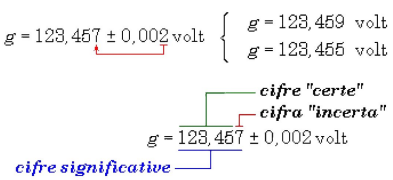
\includegraphics[scale=0.9]{Cifre Significative.png}
\end{center}
Le cifre significative del valore di una misura sono tutte quelle “certe” e la prima “incerta".\\\\
\textbf{Concetto di digit}\\
Il digit può essere definito come l'ultima cifra significativa (LSD).
Lo comprendo con un esempio:\\
Se il voltmetro mi da come risultato 1.350V ed ho come incertezza $\Delta G \pm (1\% $lettura $ + 2$ digit), significa che dovrò aggiungere 2 mV all'$1\%$ della lettura.\\\\
\subsection{Propagazione dell'incertezza nelle misure indirette}
Quando non è possibile misurare direttamente il parametro di cui si cerca la misura, la 
misurazione si ottiene attraverso la misurazione di altri parametri dai quali il misurando dipende 
attraverso leggi conosciute: si parla in questo caso di “misure indirette” in quanto la misurazione 
ha luogo non sull’incognita, ma su altre grandezze delle quali l’incognita è funzione. \\\\
\textbf{Funzioni di singola variabile } \\
se il legame fra l’incognita g ed il parametro misurato a viene espresso dalla generica 
funzione f (g=f(a)), il valore del misurando go si ottiene calcolando il valore della funzione 
in corrispondenza del valore misurato (indicato con il pedice 0) di a: 
\begin{equation}
    g_{0}=f(a)\vert_{a=a_{0}}
\end{equation}
Per individuare l'incertezza della misura indiretta si può utilizzare lo sviluppo in serie della 
funzione f sostituendo all'incremento della variabile indipendente il valore della sua 
incertezza assoluta.\\ Se l’incertezza assoluta $\Delta g$ ha un valore basso tale da poter essere 
trascurato e il valore della derivata prima della f in $a_{0}$ non è nullo, allora si può 
approssimare utilizzando la forma linearizzata:
\begin{equation}
    \Delta g \cong \left| \frac{df(a)}{da}\vert_{a=a_{0}} \right| \Delta a
\end{equation}
Perchè la prendo in modulo? Perchè l'incertezza assoluta è l'ampiezza dell'intervallo, che è sempre positiva !!!
\newpage
\noindent
\textbf{Funzione di due o più variabili }\\
Se il legame fra l’incognita g e le grandezze a e b viene espresso dalla generica funzione f 
(g=f(a,b)), il valore del misurando si ottiene calcolando il valore della funzione in 
corrispondenza dei valori misurati (indicati col pedice 0) delle due grandezze a e b
\begin{equation}
    g_{0}=f(a,b)\vert_{a=a_{0},b=b_{0}}
\end{equation}
Anche in questo caso, si può individuare l'incertezza attraverso lo sviluppo in serie della 
funzione, tenendo conto di 2 ipotesi restrittive: 
\begin{enumerate}
    \item Le incertezze di a e b non sono correlate 
    \item Le incertezze $\Delta a$ e $\Delta b$ hanno valore talmente piccolo da poter essere trattate come 
infinitesimi 
\end{enumerate}
L'incertezza assoluta può essere ricavata dallo sviluppo in serie della funzione f(a,b) 
nell’intorno del punto ($a_{0}, b_{0}$) in cui gli incrementi delle variabili a e b vengono sostituiti 
dalle rispettive incertezze assolute e tutti i termini vengono presi col segno positivo.\\ Se 
non si annullano le derivate parziali prime, la espressione della incertezza può essere 
troncata ai termini del primo ordine approssimando la funzione con la sua forma 
linearizzata:
\begin{equation}
    \Delta g \cong \pm \vert \frac{\partial f(a,b)}{\partial a}|_{a=a_{0},b=b_{0}} \Delta a+|\frac{\partial f(a,b)}{\partial b}|_{a=a_{0},b=b_{0}}
\end{equation}
\textbf{Regole pratiche per la stima dell’incertezza nelle misure derivate attraverso le operazioni elementari}
\begin{equation}
    g=a+b \Rightarrow \Delta g = \pm |\Delta a|+|\Delta b|
\end{equation}
\begin{equation}
    g=a-b \Rightarrow \Delta g = \pm |\Delta a|+|\Delta b|
\end{equation}
\begin{equation}
    g=ab \Rightarrow \Delta g = \pm |\frac{\Delta a}{a}|+|\frac{\Delta b}{b}|
\end{equation}
\begin{equation}
    g=\frac{a}{b} \Rightarrow \Delta g = \pm |\frac{\Delta a}{a}|+|\frac{\Delta b}{b}|
\end{equation}\\
\textbf{Errori di perturbazione e di consumo }\\
Ad un esame superficiale si potrebbe pensare che il circuito che descrive la misurazione della 
tensione di un segnale sia come quello in Figura \ref{fig:Circuito Misurazione Tensione} (a).\\
In realtà il misurando viene alterato per la presenza dello strumento: lo schema che rappresenta 
correttamente tale fenomeno vede l'uso del generatore eq. di Thevenin del segnale e la presenza esplicita della resistenza di ingresso (non infinita) del voltmetro (Figura \ref{fig:Circuito Misurazione Tensione} (b))\\
\begin{figure}
     \begin{subfigure}[]{}
         \centering
         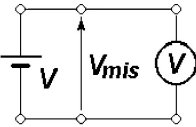
\includegraphics[scale=0.67]{Circuito Misurazione Tensione 1.png}
         \label{fig:CircuitoMisurazioneTensione}
     \end{subfigure}
     \hfill
      \begin{subfigure}[]{}
         \centering
         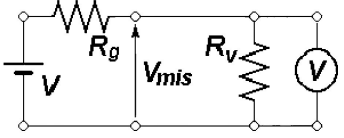
\includegraphics[scale=0.67]{Circuito Misurazione Tensione 2.png}
         \label{fig:CircuitoMisurazioneTensionee}
     \end{subfigure}
     \caption{Circuito misurazione tensione ideale e reale}
     \label{fig:Circuito Misurazione Tensione}
\end{figure}
Risolvendo lo studio teorico del circuito si ottiene l’espressione dell’alterazione inteodotta sia in termini assoluti, sia in termini relativi a V. \\
L’alterazione introdotta per la presenza dello strumento viene chiamata errore di perturbazione o errore di consumo. L'errore di consumo diminuisce all'aumentare del rapporto $\frac{R_{v}}{R_{g}}$.\\
\newpage
\section{Conversione AD}
\textbf{Segnale analogico}: funzione del tempo che è definita per ogni valore del tempo (cioè continua nel 
dominio) e continua. \\\\
\textbf{Segnale digitale}: funzione di “tempo discreta” e “quantizzata”: dunque risulta definita solamente 
in un insieme numerabile di istanti equispaziati e dotata di un codominio costituito da un insieme 
discreto di valori (non passa da una valore all'altro attraversando tutti i valori intermedi). \\\\
I segnali digitali hanno una maggiore reiezione ai disturbi rispetto ai segnali analogici (potendo 
quest'ultimi assumere infiniti valori), possono essere elaborati più facilmente dei segnali analogici 
e possono essere registrati in maniera più fedele e stabile nei segnali analogici. \\\\
La conversione A/D richiede 3 fasi successive: 
\begin{enumerate}
    \item Campionamento - discretizzazione del tempo 
    \item Quantizzazione — discretizzazione dell’ampiezza 
    \item Codifica — uso di “parole” binarie per esprimere il valore del segnale
\end{enumerate}
\textbf{Campionamento}\\
Campionare un segnale analogico significa prelevare da questo una successione temporale di 
valori costituita dalla successione dei valori istantanei assunti dal segnale in corrispondenza di 
particolari istanti, detti "istanti di campionamento". \\
L'intervallo che separa due successivi istanti di 
campionamento viene chiamato "\textbf{periodo di campionamento}" $T_{c}$ ed il suo reciproco, indicato 
come $f_{c}$, è la "\textbf{frequenza di camp.}". \\ Si potrebbe essere indotti a pensare 
che il campionamento provochi una riduzione del contenuto informativo del segnale analogico in 
quanto si perde l'informazione sul valore assunto dal segnale in tutti gli istanti diversi da quelli di 
campionamento. \\
Il teorema del campionamento ci dice invece che, in condizioni ideali, la esecuzione del 
campionamento non provoca perdita di informazione. \\\\
\underline{Teorema del campionamento o di Shannon}: se la trasformata di Fourier di un segnale a(t) è nulla per tutte le frequenze maggiori di una data frequenza $f_{max}$ allora il segnale continuo a(t) può 
essere ricavato dalla conoscenza dei suoi valori campionati (non c'è perdita d'informazione).\\ Affinché la ricostruzione sia possibile è 
indispensabile che il campionamento permetta l'acquisizione di infiniti campioni separati l'un 
l’altro da intervalli che devono avere durata inferiore al valore $\frac{1}{2}f_{max}$.\\ 
Campionare dunque significa individuare la successione di valori istantanei (ordinate) assunti da f(t) negli 
istanti di campionamento equispaziati $g(t_{0}+nT_{C})$. \\
Dalla successione ricavata mediante il teorema del campionamento, è possibile ricavare univocamente il segnale analogico g(t) se questo ha: 
\begin{itemize}
    \item Banda limitata 
    \item $T_{C}$ minore di un valore di un valore prefissato che dipende da f(t): $f_{c} > 2$W (frequenza di Nyquist)
    \item Se si acquisiscono infiniti campioni (problemone)
\end{itemize}
Un valore troppo alto di $T_{c}$ o troppo basso di $f_{c}$, provoca il fenomeno dell’alis , cioè la 
sovrapposizione delle repliche dello spettro originale nel segnale campionato: in questo caso non è possibile ricavare il segnale originale avendo a disposizione quello campionato.
\newpage
\noindent
\textbf{Quantizzazione}\\
Per quantizzare il segnale devo prima definire il "campo di misura", cioè un intervallo di valori entro cui il segnale deve 
mantenersi per permettere una corretta quantizzazione, seguendo due alternative: 
\begin{itemize}
    \item Campo unipolare con estremo inferiore nullo ed estremo superiore $E_{c}$ 
    \item Campo bipolare con estremo inferiore -$E_{c}$ ed estremo superiore +$E_{c} (simmetrici)$ 
\end{itemize}
Definito il campo di misura lo si deve suddividere in un numero arbitrario, ma finito, di intervalli 
contigui, secondo due alternative: 
\begin{itemize}
    \item Suddivisione in intervalli di ampiezza costante: quantizzazione uniforme 
    \item Suddivisione in intervalli di ampiezze diverse: quantizzazione non uniforme
\end{itemize}
Si individua poi il valore centrale di ciascun intervallo in cui è stato suddiviso il campo di misura e si 
sostituisce al valore di ciascun campione del segnale campionato $g(t_{0}+nT_{c})$, il valore centrale dell'intervallo in 
cui esso si trova. \\\\
\underline{Incertezza di quantizzazione}: La alterazione che al massimo può essere apportata al valore di 
ciascun campione è pari alla semi-ampiezza dell'intervallo entro cui il valore del campione 
(analogico) si trova.\\ Se si indica con il simbolo $e$ l'ampiezza dell'intervallo, l'incertezza introdotta 
dalla fase di quantizzazione (chiamata "incertezza di quantizzazione") risulta 
\begin{equation}
    \Delta g= \frac{2E_{c}}{2N}=\frac{E_{c}}{N}
\end{equation}\\
E' evidente che la incertezza di quantizzazione può essere ridotta agendo sia sull'ampiezza del 
campo di misura, sia sul numero degli intervalli in cui questo viene suddiviso con quantizzazione 
uniforme.\\
Più gli intervalli sono piccoli, minore è la perdita d'informazione, quindi la soluzione sarebbe dividere il campo di misura in un numero estremamente elevato di intervalli.\\
Nel caso ciò non è possibile, si praticano quantizzazioni non uniformi basate sullo studio 
statistico dell'andamento del segnale. \\\\
\underline{Schemi pratici per la quantizzazione uniforme}
\begin{itemize}
    \item Quantizzazione non silenziata: il campo è suddiviso in un numero pari di intervalli di uguale 
ampiezza dei quali una coppia (quella centrale) abbia come estremo comune lo zero.\\ In 
questa forma si ha un numero pari di intervalli, l'effettivo campo di misura si estende da - 
$E_{c}$ a +$E_{c}$ e l'ampiezza del singolo intervallo è fornito dal rapporto tra l'ampiezza del campo 
di misura (+2$E_{c}$) ed il numero N di intervalli creati. \\
Il principale difetto sta nel fatto che un campione prelevato dal segnale che ha valore nullo 
verrebbe comunque associato sempre ad un valore non nullo positivo o negativo in 
funzione del contributo del rumore e dall’offset dei dispositivi usati e quindi verrebbe quantizzato in maniera errata.
    \item Quantizzazione silenziata: il campo è suddiviso in un numero dispari di intervalli, tutti di 
uguale ampiezza salvo i due stremi e con un intervallo centrato sullo zero. \\Questa 
soluzione permette di avere un intervallo “centrato” sullo zero, pertanto tutti quei 
campioni prelevati dal segnale di ingresso a cui si sovrappone un rumore compreso 
nell'intervallo centrato appunto sullo zero, verranno associati a 0. \\
\end{itemize}
\textbf{Codifica}\\
La fase di codifica associa a ciascuno dei valori quantici corrispondenti ai centri degli N intervalli in cui è stato suddiviso il campo di misura una “parola” binaria a M bit.\\
È necessario che ciascuno degli N  valori quantici disponga di una “sua” parola, quindi non ci devono essere codifiche doppie pertanto è richiesto che:
\begin{equation}
   N\leq 2^M
\end{equation}
La scelta della strategia di corrispondenza fra la successione degli intervalli e la successione delle parole binarie è dettata da considerazioni riguardanti le codifiche più diffuse nei sistemi a microprocessore (binario puro, binario con offset, binario con offset complementato ad uno, ecc.)\\
Quello che mi interessa è come fare una \textbf{mappatura ottimale per una quantizzazione silenziata} (dato che la non silenziata è un generatore di rumore) e  avendo necessità di fare un numero dispari di intervalli, perdo uno degli elementi della mia codifica:
\begin{equation}
    N=2^M-1
\end{equation}
e quindi ci sarà un lieve incremento nella incertezza di quantizzazione perchè non sfrutto a pieno tutti i bit che uso nella mia parola, ma perdo un intervallo:
\begin{equation}
    e=\frac{2E_{c}}{N}
\end{equation}
Come posso risolvere questo problema? C'è un trucco: parto da una quantizzazione uniforme non silenziata e poi traslo di mezza ampiezza di un intervallo, mezza frontiera in basso !!!
\begin{figure}
    \centering
    \includegraphics[scale=0.8]{Sample-Hold.png}
    \caption{Circuito Sample-Hold}
    \label{fig:my_label}
\end{figure}
\subsection{Conversione AD Reale: Dispositivi}
\subsubsection{Campionatore: Sample\&Hold}
Il circuito sample and hold (abbreviato S\&H) è un campionatore utilizzato come interfaccia tra un 
segnale analogico che varia velocemente nel tempo e un dispositivo successivo, spesso un 
convertitore analogico-digitale (ADC, analog to digital converter).\\
\newpage
\noindent
I componenti principali di un S\&H sono:
\begin{itemize}
    \item Due OPAMP connessi come "inseguitore di tensione" (guadagno unitario)
    \item Un MOSFET che opera come "interruttore" 
    \item Un C che opera come "memoria"
\end{itemize}
\begin{figure}
\begin{subfigure}[]{}
   \centering
    \includegraphics[scale=0.5]{S&H Ideale.png}
    \label{fig:S&H Funzionamento ideale}
\end{subfigure}
\hfill
\begin{subfigure}[]{}
   \centering
   \includegraphics[scale=0.5]{Acquisition Time.png}
   \label{fig:S&H Funzionamento Reale}
\end{subfigure}
\hfill
\begin{subfigure}
   \centering
   \includegraphics[scale=0.5]{Droop Rate.png}
   \label{fig:Droop Rate}
\end{subfigure}
        \caption{Funzionamento S\&H}
        \label{fig:Sample}
\end{figure}
L'effetto di questo circuito è di 
mantenere il valore analogico costante per il tempo necessario al convertitore o ad altri circuiti 
successivi per compiere delle operazioni sul segnale. \\
Nella maggior parte dei circuiti si utilizza un condensatore a bassa capacità C per conservare la 
tensione analogica, più un interruttore (costituito solitamente da un MOSFET, che ha una piccola 
resistenza di ingresso intrinseca R), il quale connette e disconnette il condensatore all'ingresso 
analogico.\\
Al source del transistor è collegato un buffer che mantiene l'impedenza di ingresso 
globale elevata.\\
La procedura di utilizzo consiste nell'iniettare nel gate del transistor un segnale 
impulsivo, permettendo così al source del MOSFET di raggiungere (in modo pressoché istantaneo, 
date le grandezze del partitore RC) la tensione del generatore in ingresso.\\
Nell'istante successivo all'immissione dell'impulso, l'interruttore si chiude, perciò il condensatore non si scarica, 
"memorizzando" così il segnale di ingresso.\\
Ripetendo tale procedura più volte, si ottiene in uscita 
una rappresentazione "a scalino" della tensione di ingresso.\\
La frequenza con cui l'interruttore 
viene aperto o chiuso è la frequenza di campionamento del sistema.
Quindi idealmente, un S\&H si comporta come in FIG \ref{fig:Sample}(a)\\\\
\textbf{Comportamento Reale: Acquisition Time}\\
Vado ora a vedere il comportamento reale inserendo il concetto di "Acquisition Time": una volta finita la fase di mantenimento (HOLD) attivo l'inseguimento rendendo conduttore il MOSFET, ma il MOSFET non ha una R nulla, di conseguenza le cariche che devono arrivare sul C per far su che la tensione faccia un salto, non possono arrivare in un tempo nullo, ci sarà un transitorio di carica!!! (FIG \ref{fig:Sample}(b))\\\\
\textbf{Comportamento Reale: Ricombinazione delle Cariche}\\
A causa  della resistenza d'interdizione del MOSFET, dalle $R_{IN}$ dell'OPAMP, che nel caso reale sono diverse da zero, durante la fase di HOLD, la tensione ai capi del condensatore non è costante, dato che il C si scarica sulla $R_{P}$ (che schematizza la resistenza del MOSFET e dell'OPAMP) con legge esponenziale.\\
La misura della velocità di scarica a avviene tramite il DROOP RATE, che è definito come la tangente alla curva di scarica del condensatore. (FIG \ref{fig:Sample} (c))
\begin{equation}
    tg(\alpha)=\text{DROOP RATE} 
\end{equation}
\newpage
\noindent
\textbf{Comportamento Reale: Droop Voltage}\\
Dato che la tensione $V_{OUT}$ non è costante durante la fase di HOLD, è possibile definire la variazione a causa della scarica del condensatore attraverso il DROOP VOLTAGE.\\
Dato che maggiore è il valore di C e minore sarà rilevante la perditsa di carica durante la fase di scarica, si può dire che il DROOP sia inversamente proporzionale al valore della capacità:
\begin{equation}
   \text{DROOP}=\frac{1}{C} \text{   (anche uguale alla banda passante)}
\end{equation}
Il DROOP è accettabile fintanto che risulta la metà dell'ampiezza degli intervalli di quantizzazione, pertanto è possibile dare un'espressione approssimata del DROOP VOLTAGE:
\begin{equation}
    \text{DROOP VOLTAGE}=\text{DROOP RATE}(t-t_{0})
\end{equation}
\textbf{Caso Reale: Sottrazione delle Cariche}\\
Quando il dispositivo passa dalla fase di TRACK, alla fase di HOLD, la polarità tra Gate e Source deve essere invertita, il che si traduce nel dover invertire anche la polarità del condensatore parassita.\\
Affinchè la piastra superiore sia ad un potenziale più elevato di quella inferiore durante la fase di HOLD, il C parassita ruba cariche positive dal C di memoria e pertanto la $V_{OUT}$ scende leggermente, fornendo un PEDESTAL.\\\\
\textbf{Come scelgo il valore della capacità per il C di memoria?}\\
Aumentare C provoca:
\begin{itemize}
    \item Diminuzione “droop –rate”  (+)
    \item Diminuzione “pedestal” (+)
    \item Aumento “acquisition time” (-)
    \item Diminuzione frequenza di taglio e banda passante (-)
\end{itemize}
\begin{figure}
\begin{subfigure}
   \centering
    \includegraphics[scale=0.59]{Droop Voltage.png}
    \label{fig:droop Voltage}
\end{subfigure}
  \hfill
  \begin{subfigure}
     \centering
    \includegraphics[scale=0.59]{Pedestal Schema.png}
    \label{fig:pedestal schema}
  \end{subfigure}
  \hfill
 \begin{subfigure}
    \centering
    \includegraphics[scale=0.59]{Pedestal Grafico.png}
    \label{fig:pedestal grafico}
 \end{subfigure}
 \caption{Droop Voltage e Pedestal}
  \label{fig:droop}
\end{figure}
\subsubsection{Convertitore AD Flash o "Parallelo"}

\end{document}
